% To create a slide, use the following:
% \begin{frame}{TITLE}
%     BODY
% \end{frame}

% To create a slide with a bullet list, use the following:
% \begin{frame}{TITLE}
%     \begin{itemize}
%         \item ITEM 1
%         \item ITEM 2
%     \end{itemize}    
% \end{frame}

\begin{frame}{CSE 145 Updates: Birdclef submissions}
    \centering
    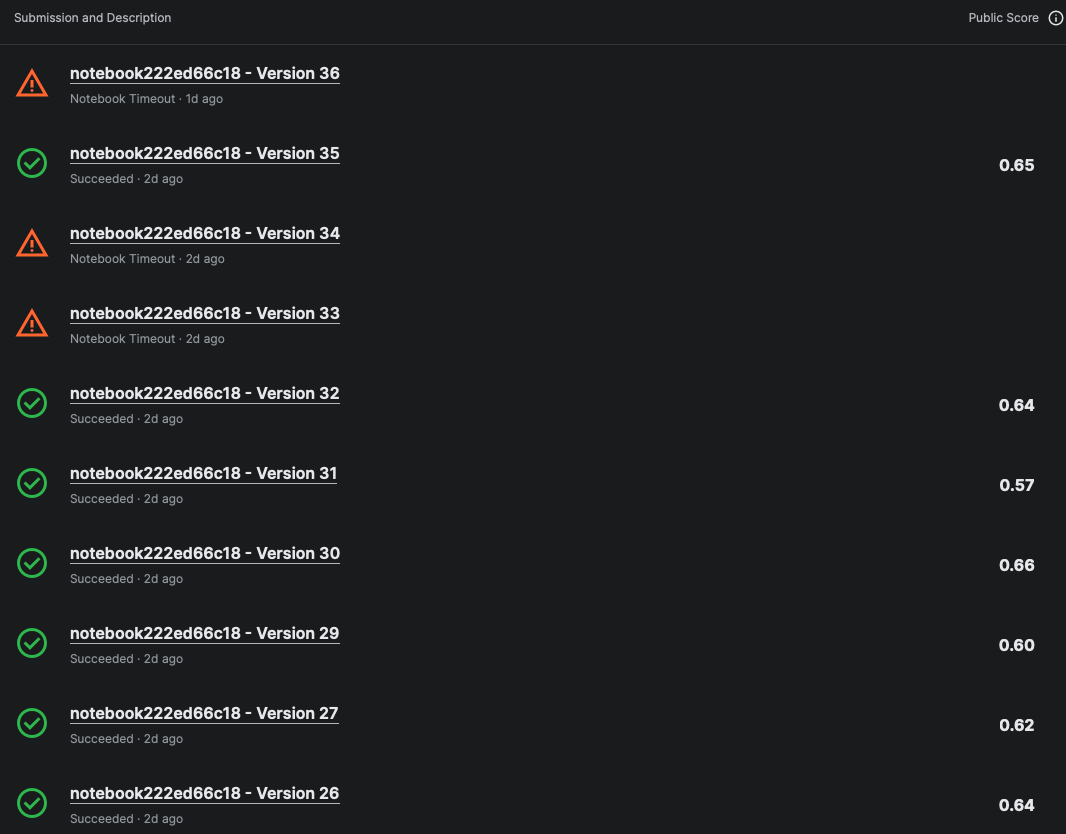
\includegraphics[height=0.7\textheight,width=0.7\textwidth,keepaspectratio]{images/Birdclef_submissions.png}
\end{frame}

% To create a slide with numbered list, use the following:
\begin{frame}{CSE 145 Updates}
    \begin{enumerate}
        \item Model submissions via Kaggle are working
        \item Currently working on Rust implementation
        \item Running ensemble after Rust implementation
        \item Mamba model finished training - evaluation
        \item Working on the final report
    \end{enumerate}
\end{frame}

% To create a slide with a graphic:
% 1. Add the graphic to this folder (named picture.png)
% 2. Use the following:


% To create a slide with two columns, use the following:
% \begin{frame}{TITLE}
%     \begin{columns}
%         \begin{column}{0.5\textwidth}
%             COLUMN 1 BODY
%         \end{column}
%         \begin{column}{0.5\textwidth}
%             COLUMN 2 BODY
%         \end{column}
%     \end{columns}
% \end{frame}
